\documentclass[notheorems]{beamer}
\usetheme{Lab2C}
\usepackage{graphicx}
\usepackage{subcaption}
\usepackage{amsfonts}
\usepackage{amsmath}
\usepackage{amssymb}
\usepackage{amsthm}
\usepackage{algorithm}
\usepackage{algorithmic}
\usepackage{bm}
\usepackage{hyperref}
\usepackage{footmisc}
\usepackage{xcolor}




\DeclareMathOperator*{\argmin}{arg\,min}
\DeclareMathOperator*{\argmax}{arg\,max}
\DeclareMathOperator\E{\mathbb{E}}
\DeclareMathOperator\Var{\mathrm{Var}}
\def\R{\mathbb{R}}
\def\P{\mathcal{P}}
\usepackage{mathtools}
\DeclarePairedDelimiter\abs{\lvert}{\rvert}
\DeclarePairedDelimiter\norm{\lVert}{\rVert}
\DeclarePairedDelimiter\inner{\langle}{\rangle}
\DeclarePairedDelimiter\floor{\lfloor}{\rfloor}
\DeclarePairedDelimiter\ceil{\lceil}{\rceil}
\def\red#1{\textcolor{red}{#1}}
\makeatletter
\newcommand{\algorithmicfunction}{\textbf{function}}
\newcommand{\algorithmicendfunction}{\algorithmicend\ \algorithmicfunction}
\newenvironment{ALC@func}{\begin{ALC@g}}{\end{ALC@g}}
\newcommand{\FUNCTION}[2][default]{\ALC@it\algorithmicfunction\ #2\ %
\textbf{:}%
\ALC@com{#1}\begin{ALC@func}}
\ifthenelse{\boolean{ALC@noend}}{
    \newcommand{\ENDFUNCTION}{\end{ALC@func}}
  }{
    \newcommand{\ENDFUNCTION}{\end{ALC@func}\ALC@it\algorithmicendfunction}
  }
\makeatother
\theoremstyle{definition}
\newtheorem{definition}{Definition}
\newtheorem{theorem}{Theorem}
\newtheorem{example}{Example}
\newtheorem{proposition}{Proposition}
\newtheorem{corollary}{Corollary}
\newtheorem{lemma}{Lemma}
\newtheorem{remark}{Remark}

\newif\ifbeamer
\beamertrue

\title{Info-Detection: An Information-Theoretic Approach to Detect Outlier}
\author{Feng Zhao\inst{1} \and Fei Ma\inst{2}\and Yang Li\inst{2} \and Shao-Lun Huang\inst{2} \and Lin Zhang \inst{1,2}}
\institute{\inst{1}Dept. of Electronic Engineering, Tsinghua University
\and \inst{2}Tsinghua-Berkeley Shenzhen Institute, Tsinghua University}
\date{\today}
\begin{document}
\begin{frame}
	\titlepage
\end{frame}
\section*{Outline}
\begin{frame}
	\tableofcontents
\end{frame}

\section{Introduction}
\subsection{Outlier detection and existing method}
\begin{frame}
\frametitle{Outlier detection}
	\begin{columns}
		\column{5cm}
		\begin{figure}
			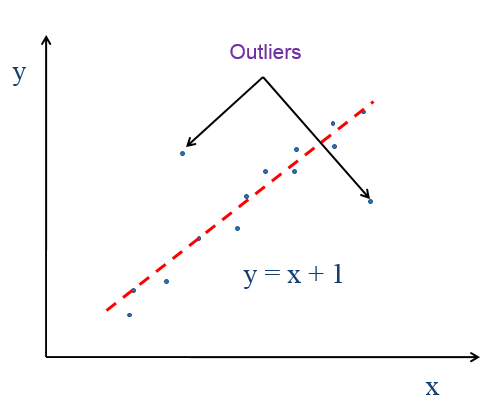
\includegraphics[width=4cm]{pic/outlier_detection_intro.png}
		\end{figure}
		\column{5cm}
		Outlier detection is the identification of abnormal data which differs from the majority of the data.
	\end{columns}
\begin{figure}
	\centering
	\begin{subfigure}{0.33\textwidth}
		
\includegraphics[width=\textwidth]{pic/fraud_detection.jpg}
		\caption{Fraud Detection}
	\end{subfigure}~~~~~
	\begin{subfigure}{0.33\textwidth}
		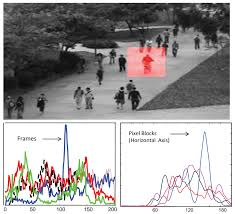
\includegraphics[width=\textwidth]{pic/activity_monitoring.jpg}
		\caption{Activity Monitoring}
	\end{subfigure}
\end{figure}  
\end{frame}
\begin{frame}
\frametitle{Existing Method}
\begin{figure}
	\centering
	\begin{subfigure}{0.33\textwidth}
		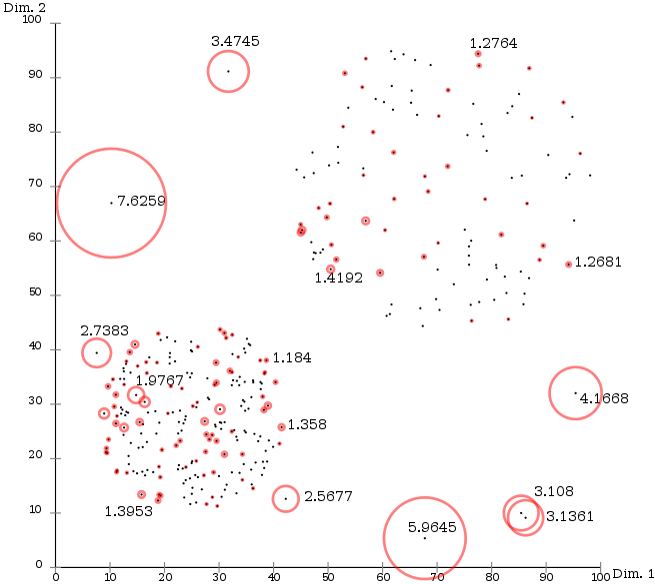
\includegraphics[width=\textwidth]{pic/lof.png}
		\caption{Local Outlier Factor}
	\end{subfigure}~
	\begin{subfigure}{0.58\textwidth}
		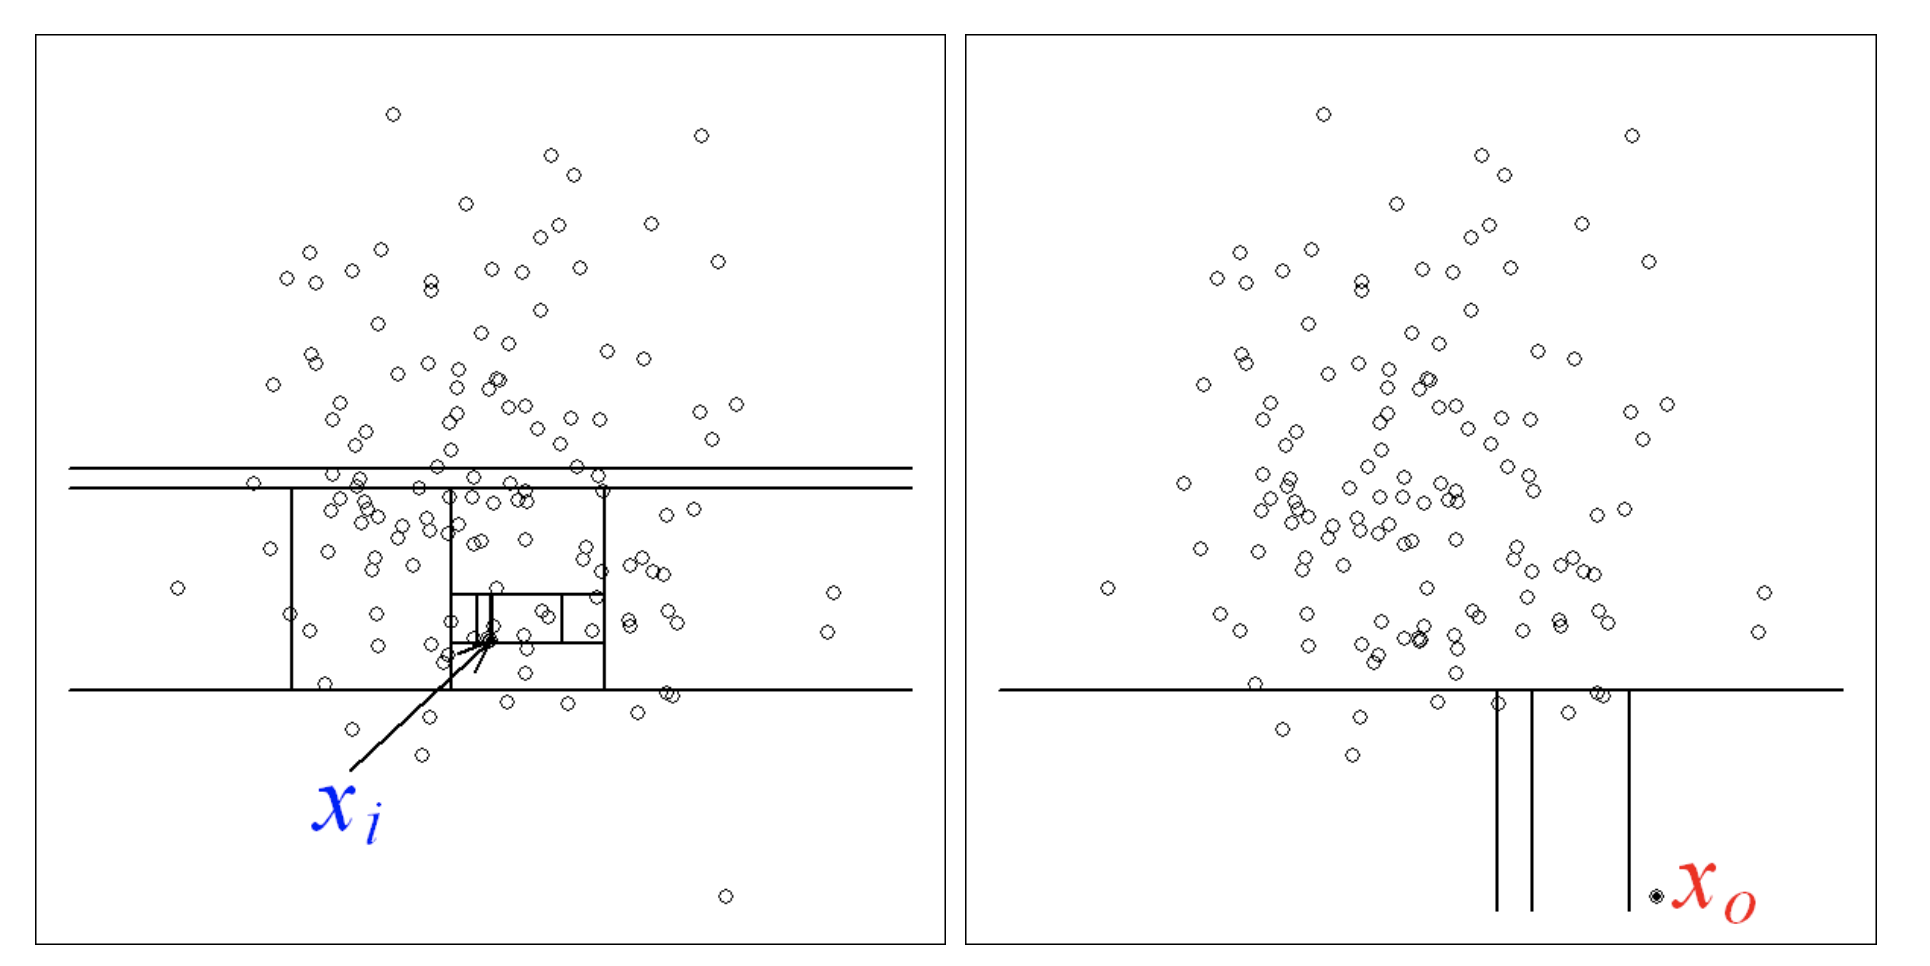
\includegraphics[width=\textwidth]{pic/if.png}
		\caption{Isolation Forest}
	\end{subfigure}
\end{figure}  
	\begin{columns}
\column{0.4\textwidth}
\begin{figure}
		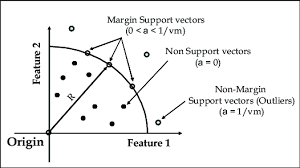
\includegraphics[width=4.5cm]{pic/one_class_svm.png}
		\caption*{ \textcolor{thupurple}{(c)} One class SVM}
\end{figure}
\column{0.6\textwidth}
\quad Shortcomings:
\begin{itemize}
\item the number of outliers needs to known 
\item hyperparameters matter
\end{itemize}
\end{columns}
\end{frame}
\subsection{Related work}
\begin{frame}
	\frametitle{Related work}
\begin{itemize}
\item Cluster based method
	\begin{enumerate}
		\item Campello et al. in 2015 proposed a hierarchical density estimate method \cite{RN432}
%to do outlier detection
		\item Nagano et al in 2010 proposed a minimum average cost clustering method \cite{mac}
%which shares the same hierarchical clustering structure with info-clustering.
		\item Chan C et al. in 2016 proposed info-clustering method \cite{ic}
%which is a hierarchical clustering method.
	\end{enumerate}
\item Graph partition algorithm
\begin{enumerate}
\item Narayanan in 1991 proposes an algorithm to compute the principal sequence of partition \cite{psp}
\item Kolmogorov in 2010 proposes a parametric algorithm for the same task \cite{pmf}
\end{enumerate}
\end{itemize}
Our work
\begin{itemize}
\item Info-Detection method
\item Improved algorithm for principal sequence of partition
\end{itemize}
\end{frame}
\section{Formulation of Info-Detection}
\subsection{Info-Clustering}
\begin{frame}
\frametitle{Review of Info-Clustering}
\begin{enumerate}
\item directed graph $G(V, E)$; Node set $Z_V=\{Z_i | i \in V\}$
\item partition $\P=\{C_1, \dots, C_k\}, \bigcup_{i=1}^k C_i = V$ and $i\neq j \Rightarrow C_i \cap C_j = \emptyset$
\item $\Pi$ is the collection of all partitions of $V$, $\Pi' = \Pi \backslash \{V\}$
\item $f(\cdot)$ is the graph in-cut function, $f(C)=\sum_{i \neq C, j\in C, (i,j) \in E} w_{ij}$
\item $f[\cdot]$ is a function defined on $\Pi$ by $f[\P]=\sum_{C\in \P}f(C)$
\end{enumerate}
\begin{definition}[info-cluster]
Given $G(V, E)$, the cluster set $C_{\gamma}(Z_V)$ is defined as 
\begin{align}
I_{\mathcal{P}}(Z_V) & = \frac{f[\P]}{ \abs{\mathcal{P}} - 1}\\
I(Z_V) & = \min_{\mathcal{P} \in \Pi'(V)} I_{\mathcal{P}}(Z_V) \\
C_{\gamma}(Z_V) & := \textrm{maximal}\{ B \in V \vert \, \abs{B} > 1, I(Z_B) > \gamma \}
\end{align}
\end{definition}
\end{frame}
\begin{frame}{Review of Info-Clustering}
\begin{enumerate}
\item  every two sets $C(Z_V)=\bigcup_{\gamma \geq 0} C_{\gamma}(Z_V)$ are either disjoint or have subset relationship
\item sets from $C(Z_V)$ can be arranged in a clustering tree $\mathcal{T}$; The leaf node of $\mathcal{T}$ is $\{j\}$.
\item the largest threshold value $\gamma_N = \max_{A\subseteq V, \abs{A}>1} I(Z_A)$; The maximal set to achieve this is denoted $B$; $\gamma_N = I(Z_B)$.
\end{enumerate}
Example
\begin{columns}
\column{0.45\textwidth}
\begin{figure}
		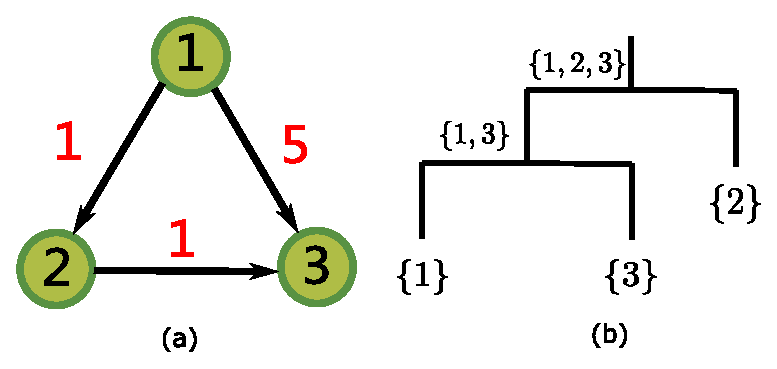
\includegraphics[width=4.5cm]{pic/example_directed.eps}
\end{figure}
\column{0.55\textwidth}
	\begin{equation*}
	C_{\gamma}(Z_V)	=\begin{cases}
					\{\{1,2,3\}\} & \gamma < 2 \\
					\{\{1,3\}\} & 2\leq \gamma < 5 \\
					\emptyset & \gamma \geq \gamma_N = 5
		\end{cases}
	\end{equation*}
\end{columns}
\end{frame}
\subsection{Info-Detection}
\begin{frame}
	\frametitle{Info-Detection Method}
\begin{itemize}
\item For $\gamma_N = I(Z_B)$, nodes in $B$ are inliers and nodes in $V\backslash B$ are outliers.
\item The ourlier score $Z_j$ for $j \in V\backslash B$ is measured with the depth of the set $\{j\}$ in the hierarchical tree.
\end{itemize}
Example
	\begin{figure}
		\centering
		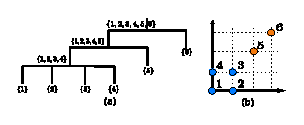
\includegraphics[width=9cm]{pic/outlier_example.eps}
		\caption*{Info-Detection applied to 6 points on Cartesian plane, with $w_{ij} = \exp(-d_{ij}^2)$}\label{fig:ex}
	\end{figure}
\end{frame}
\begin{frame}{Prediction Scheme for Info-Detection}
For newly added node $i'$. Let $V'=B\cup \{i'\}$, we can compute $\gamma'_N$ for $G(V', E(V'))$.
$ \gamma'_N > \gamma_N \iff i'$ is normal observation. We found that
\begin{proposition}
\begin{equation}
\gamma'_N > \gamma_N \iff  \sum_{i \in B} w_{ii'} > \gamma_N 
\end{equation}
\end{proposition}
\begin{figure}
	\centering
	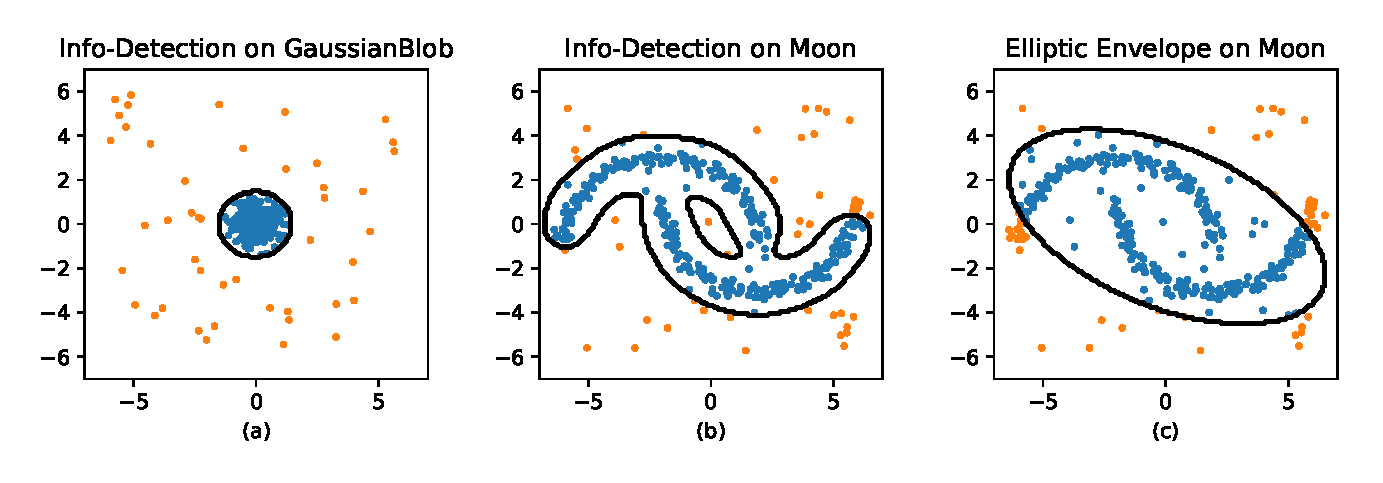
\includegraphics[width=\textwidth]{pic/outlier_boundary_illustration.eps}
	\caption*{Detection boundary lines}	\label{fig:boundary}
\end{figure}
\end{frame}

\section{Algorithms}
\frame{\tableofcontents[currentsection]}
\begin{frame}{Review of Principal Sequence of Partition}
It has been found the mathematical structure of info-clustering is the same with that of principal sequence of partition.
\begin{definition}[Principal Sequence of Partition]
\begin{align}
h_{\P}(\lambda) &=  f[\P] - \abs{\P} \lambda  \label{eq:hPL}\\
h(\lambda) &= \min_{\P \in \Pi'(V)} h_{\P}(\lambda) \label{eq:hLambda}
\end{align}
The optimal partitions $\P_1, \dots, \P_k$ for $h(\lambda)$ are nested such that $\P_1 \succeq \P_2 \dots \succeq \P_k$,  which are called principal sequence of partition (PSP) of the graph $G$.
\end{definition}
We call $\lambda^*$ a critical value for PSP if $\P_i, \P_{i+1}$ are both minimizer for $h(\lambda^*)$ in \eqref{eq:hLambda}.
The largest critical value is equal to $\gamma_N$ and the largest set in $\P_{k-1}$ is equal to $B$.
\end{frame}
\begin{frame}
\frametitle{Review of Narayanan's Algorithm to compute PSP}
\begin{columns}
\column{0.5\textwidth}
\algsetup{linenosize=\tiny}
\begin{algorithm}[H]
\caption*{Narayanan's Algorithm}\label{alg:psp}
{\tiny
\begin{algorithmic}[1]
\REQUIRE a directed graph $G(V,E)$
\ENSURE A sorted critical value array \textbf{L} and a reverse ordered array \textbf{PSP} containing $\P_1,\dots, P_k$.
\STATE \textbf{L}  $\leftarrow$ empty list.
\STATE $Q\leftarrow \{V\}, P \leftarrow \{ \{i \} | i \in V\}$
\STATE $\mathbf{PSP}= [Q, P]$
\STATE \texttt{Split}$(Q,P)$
\STATE sort $L$ and sort $\mathbf{PSP}$ with respect to $\succeq$ 
\FUNCTION{\texttt{Split}$(Q,P)$}
 \STATE\label{alg:gamma} $\gamma' = {1 \over \abs{P} - \abs{Q}} (f(P)-f(Q))$
 \STATE $h' = {1 \over \abs{P} - \abs{Q}}(\abs{P} f(Q) - \abs{Q} f(P))$
 \STATE $(\tilde{h}, P') = \texttt{DT}(f,\gamma')$
 \IF{$\tilde{h} = h'$}
 	\STATE insert $\gamma'$ to $\mathbf{L}$
 \ELSE
 	\STATE insert $P'$ to $\mathbf{PSP}$
 	\STATE \texttt{Split}$(Q, P')$
 	\STATE \texttt{Split}$(P',P)$
 \ENDIF
\ENDFUNCTION
\end{algorithmic}
}
\end{algorithm}
The whole graph $G$ is used in each compution of \texttt{DT} routine.
\column{0.5\textwidth}
Example
\begin{figure}
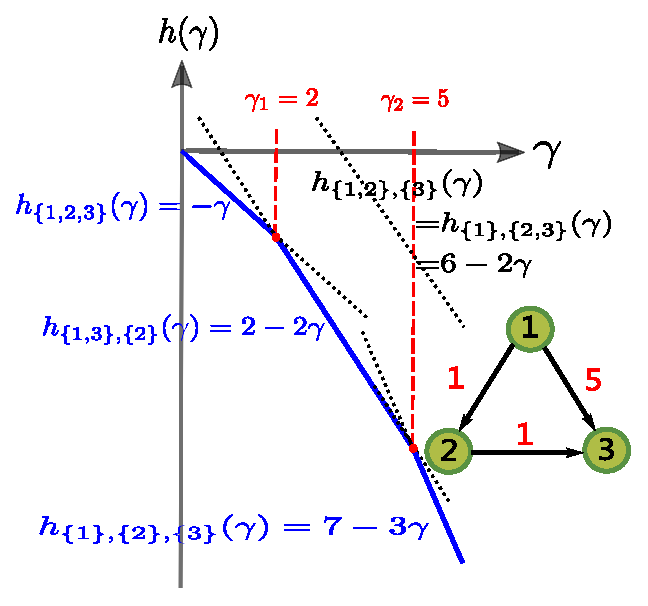
\includegraphics[width=4.5cm]{pic/dt_with_graph.eps}
\end{figure}
\begin{align*}
\P_0  & = \{\{1,2,3\}\} \\
\P_1  & = \{\{1,3\},\{2\}\} \\
\P_2  & = \{\{1\},\{2\},\{3\}\} 
\end{align*}
\end{columns}
\end{frame}
\begin{frame}
\frametitle{Improved PSP Algorithm}
\begin{columns}
\column{0.5\textwidth}
\vskip -1.2em
\algsetup{linenosize=\tiny}
\begin{algorithm}[H]
\caption*{{\footnotesize Improved PSP Algorithm}}
{\tiny
	\begin{algorithmic}[1]
		\REQUIRE a directed graph $G(V, E)$
		\ENSURE a hierarchical tree $\mathcal{T}(K, E)$ where $K \subseteq 2^{V}$ is node set and $E$ is edge set.
		\STATE initialize tree $\mathcal{T}$ with $V$ as root node, $\{j\}(j\leq \abs{V})$ as leaf node and no stem node.
		\STATE \texttt{Split}($G, V$)
		\FUNCTION{\texttt{Split}($\widetilde{G}, \widetilde{V}$)}
		\STATE $w$ is the summation of all edge weights of $\widetilde{G}$ 
		\STATE $\gamma' = \frac{w}{\abs{V(\widetilde{G})}-1}$ where $V(\widetilde{G})$ is node set of graph $\widetilde{G}$ \label{alg:gamma_apostrophe}
		\STATE $(\tilde{h}, P') = \texttt{DT}(\widetilde{G}, \gamma')$ 
		\IF{$\tilde{h} = - \gamma'$}
		\STATE add edge weight $\gamma'$ in $\mathcal{T}$ from $\widetilde{V}$ to its children
		\ELSE
		\FOR{$S$ in $P'$ and $\abs{S}>1$}
		\STATE make children of $\widetilde{V}$ in $\mathcal{T}$ have new parent $S$		
		\STATE make the parent of $S$ be $\widetilde{V}$
		\STATE \texttt{Split}($\widetilde{G}[S], S$) where $\widetilde{G}[S]$ is the subgraph of $\widetilde{G}$ restricted on $S$
		\STATE contract $S$ to a single node in $\widetilde{G}$ % graph \widetilde{G} is modified
		\ENDFOR 
		\STATE \texttt{Split}($\widetilde{G}, \widetilde{V}$)		
		\ENDIF
		\ENDFUNCTION
	\end{algorithmic}
}
\end{algorithm}
\vskip -1.2em
Smaller graph $G$ is used in each compution of \texttt{DT} routine.
\column{0.5\textwidth}
Example
\begin{figure}
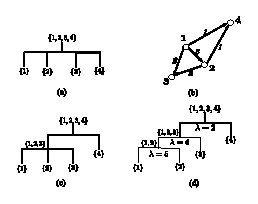
\includegraphics[width=5cm]{pic/alg_illustration.eps}
\end{figure}
Time complexity for dense graph
\begin{itemize}
\item Narayanan's: $O(n^5)$
\item Ours: $O(n^4)$
\end{itemize}
\end{columns}
\end{frame}

\begin{frame}
	\frametitle{Empirical Comparison for three implementation of PSP}
\end{frame}
\section{Experimental Results}
\begin{frame}
	\frametitle{Experimental Results}
\begin{table}
\centering
\begin{tabular}{ccccc}
\hline
              &  GaussianBlob   &      Moon       &  Lymphography  &     Glass     \\
\hline
   Type    & artificial & artificial & real-world & real-world \\
   N(Inliers) & 255  & 300 & 142  & 207 \\
   N(outliers)   & 45 &  45  & 6 & 7 \\
   N(features)   & 2 &  2  & 19 & 7  \\
\hline
\end{tabular}
\end{table}
\begin{itemize}
\item True Positive Rate (TPR)  $=\frac{N(\textrm{detected inliers})}{N(\textrm{inliners})} \geq 90\% $
\item True Negative Rate (TNR) $=\frac{N(\textrm{detected outliers})}{N(\textrm{outliers})}$
\end{itemize}
\begin{table}
\centering
{\scriptsize
\begin{tabular}{ccccc}
\hline
       TPR/TNR        &  GaussianBlob   &      Moon       &  Lymphography  &     Glass     \\
\hline
    Info-Detection    & 100\%/100\% &  96.7\%/82.2\%  & 97.9\%/100\% & 91.2\%/11.1\% \\
 local outlier factor & 100\%/100\% & 100\%/100\% & 98.6\%/83.3\%  & 96.6\%/22.2\% \\
   isolation forest   & 100\%/100\% &  96.7\%/77.8\%  & 99.3\%/100\% & 90.2\%/22.2\% \\
  elliptic envelope   & 100\%/100\% &  91.3\%/42.2\%  & 93.0\%/83.3\%  & 94.6\%/0.0\%  \\
    one class SVM     &  98.8\%/91.1\%  &  93.0\%/55.6\%  & 93.0\%/66.7\%  & 91.7\%/22.2\% \\
\hline
\end{tabular}
}
\end{table}

\end{frame}	
\section{Conclusion}
\begin{frame}
\frametitle{Conclusion}
\begin{itemize}
\item Formulate Info-Detection method
\item Propose improved principal sequence of partition algorithm 
\item Demonstrate Info-Detection performs well on some datasets
\end{itemize}
\end{frame}
\section*{Reference}
\begin{frame}
\frametitle{Reference}
\setbeamertemplate{bibliography item}[triangle]
\bibliographystyle{plain}
{\scriptsize
\bibliography{id}
}
\end{frame}
\end{document}
